\subsection{Overall Comparison}
\label{expsec:overall_comparison}

\begin{table}[t]
    \centering
    \caption{\bf 
    Comparison of \sys with baselines on open-source LLMs. The best and second-best results are highlighted in \textbf{bold} and \underline{underlined}, respectively.
    % Results on more LLMs (0.5B, 1.5B, 3B, 7B, 14B models of Qwen2.5 and 0.6B, 1.7B, 4B models of Qwen3) can be found in our technique report~\cite{technical_report}.
    }
    \label{tbl:opensource_exp}
    \vspace{-1em}

    % =======================================================
    % Subtable 5: Open-Source & Training - Qwen3-14B
    % =======================================================
    \begin{subtable}[t]{0.9\columnwidth}
        \centering
        \caption{\bf{Results on Qwen3-14B.}}
        \label{subtbl:open_qwen14b}
        \vspace{-0.5em}
        \resizebox{0.99\linewidth}{!}{
        \begin{tabular}{|c||c|c||c|c|c|c|}
            \hline
            \multirow{2}{*}{\textbf{Method}} & \multicolumn{2}{c||}{\textbf{Synth-Spider}} & \multicolumn{2}{c|}{\textbf{Synth-Bird}} & \multicolumn{2}{c|}{\textbf{Parrot}} \\ \cline{2-7}
             & \textbf{Acc.} & \textbf{Comp.} & \textbf{Acc.} & \textbf{Comp.} & \textbf{Acc.} & \textbf{Comp.} \\
            \hline \hline
            \multicolumn{7}{|c|}{\cellcolor{gray!10}\textit{Prompting Baselines}} \\
            % CodeGen & 41.83 & 67.08\% & 27.74 & 48.71\% & 31.52 & 86.16\% \\
            PaS & 7.67 & 20.67\% & 3.09 & 21.86\% & 9.56 & 22.36\% \\
            MCTS-OP & 21.91 & 72.56\% & 7.22 & {78.69\%} & 24.95 & 83.02\% \\
            MontePrep & 9.46 & 19.62\% & 18.63 & 38.15\% & 26.94 & 57.87\% \\
            AutoPrep & 36.75 & 71.61\% & 10.41 & 39.89\% & 28.54 & 74.05\% \\
            CodeGen & 45.47 & 68.18\% & 29.48 & 49.20\% & 30.83 & 81.08\% \\
            ReAct & 40.39 & 69.02\% & 16.04 & 46.56\% & 30.80 & 76.44\% \\
            \hline \hline
            \multicolumn{7}{|c|}{\cellcolor{gray!10}\textit{Training Methods (Only Trained on Synth-Spider)}} \\
            % IL & \underline{59.61} & \underline{88.65\%} & \underline{44.16} & 74.75\% & \underline{34.58} & 
            IL & \underline{61.70} & \underline{85.26\%} & \underline{48.01} & \underline{81.23\%} & \underline{37.95} & \underline{89.39\%} \\
            RL-GRPO & 51.22 & 77.68\% & 32.25 & 67.22\% & 35.06 & 82.9\% \\ \hline
            \begin{tabular}{@{}c@{}}\textbf{\sys}\\ \textbf{(Ours)}\end{tabular} & \textbf{67.18} & \textbf{97.21\%} & \textbf{54.09} & \textbf{92.26\%} & \textbf{40.44} & \textbf{96.41\%} \\
            \hline
        \end{tabular}
        }
    \end{subtable}

    \vspace{0.5em}
    
    % =======================================================
    % Subtable 4: Open-Source & Training - Qwen3-8B
    % =======================================================
    \begin{subtable}[t]{0.9\columnwidth}
        \centering
        \caption{\bf{Results on Qwen3-8B.}}
        \label{subtbl:open_qwen8b}
        \vspace{-0.5em}
        \resizebox{0.99\linewidth}{!}{
        \begin{tabular}{|c||c|c||c|c|c|c|}
            \hline
            \multirow{2}{*}{\textbf{Method}} & \multicolumn{2}{c||}{\textbf{Synth-Spider}} & \multicolumn{2}{c|}{\textbf{Synth-Bird}} & \multicolumn{2}{c|}{\textbf{Parrot}} \\ \cline{2-7}
             & \textbf{Acc.} & \textbf{Comp.} & \textbf{Acc.} & \textbf{Comp.} & \textbf{Acc.} & \textbf{Comp.} \\
            \hline \hline
            \multicolumn{7}{|c|}{\cellcolor{gray!10}\textit{Prompting Baselines}} \\
            % CodeGen & 29.53 & 45.22\% & 19.12 & 32.52\% & 24.25 & 56.27\% \\
            PaS & 4.68 & 7.42\% & 0.65 & 4.33\% & 3.09 & 8.32\% \\
            MCTS-OP & 12.90 & 15.19\% & 0.90 & 73.56\% & 17.33 & 23.71\% \\
            MontePrep & 8.81 & 19.97\% & 13.70 & 21.96\% & 25.95 & 56.08\% \\
            AutoPrep & 26.44 & 50.85\% & 8.52 & 42.28\% & 25.20 & 70.42\% \\
            CodeGen & 6.27 & 12.10\% & 7.47 & 15.69\% & 7.27 & 25.50\% \\
            ReAct & 29.63 & 52.59\% & 10.41 & 46.22\% & 22.11 & 57.97\% \\
            DeepAnalyze & 35.66 & 82.02\% & 1.74 & 62.17\% & 29.01 & 66.67\% \\
            \hline \hline
            \multicolumn{7}{|c|}{\cellcolor{gray!10}\textit{Training Methods (Only Trained on Synth-Spider)}} \\
            % IL & \underline{58.62} & \underline{92.63\%} & \underline{41.63} & \underline{83.98\%} & \underline{33.26} & \underline{91.36\%} \\ % 2025 Version
            IL & \underline{59.65} & \underline{90.54\%} & \underline{43.30} & \underline{80.43\%} & \underline{36.15} & \underline{91.08\%} \\
            RL-GRPO & 47.81 & 76.54\% & 29.95 & 68.69\% & 32.82 & 85.05\% \\ \hline
            \begin{tabular}{@{}c@{}}\textbf{\sys}\\ \textbf{(Ours)}\end{tabular} & \textbf{65.99} & \textbf{97.46\%} & \textbf{53.39} & \textbf{92.78\%} & \textbf{39.93} & \textbf{98.46\%} \\
            \hline
        \end{tabular}
        }
    \end{subtable}
    \vspace{-1em}
\end{table}

% \begin{table}[t]
    \centering
    \caption{\bf Comparison of \sys and baselines on SOTA LLMs. Results on more LLMs (DoubaoSeed1.6-Thinking, DeepSeek-V3.1 and DoubaoSeed1.6-flash) can be found in our technique report ~\cite{technical_report}.}
    \label{tbl:sota_exp}
    \vspace{-1em}

    % =======================================================
    % Subtable 2: SOTA - Claude-4
    % =======================================================
    \begin{subtable}[t]{\columnwidth}
        \centering
        \caption{\bf{Results on SOTA LLMs (Backbone: Claude-4).}}
        \label{subtbl:sota_claude}
        \vspace{-0.15em}
        \resizebox{0.99\linewidth}{!}{
        \begin{tabular}{|c||c|c|c|c|c|c|}
            \hline
            \multirow{2}{*}{\textbf{Method}} & \multicolumn{2}{c|}{\textbf{DP-Spider}} & \multicolumn{2}{c|}{\textbf{DP-Bird}} & \multicolumn{2}{c|}{\textbf{Parrot}} \\ \cline{2-7}
             & \textbf{Acc.} & \textbf{Comp.} & \textbf{Acc.} & \textbf{Comp.} & \textbf{Acc.} & \textbf{Comp.} \\
            \hline \hline
            CodeGen & 59.51 & 86.65\% & 50.55 & 70.27\% & 40.44 & 91.93\% \\ 
            PaS & 46.91 & 79.83\% & 27.59 & 61.55\% & 41.19 & 93.43\% \\
            MCTS-OP & 66.58 & \underline{99.05\%} & 58.91 & \underline{95.32\%} & 41.68 & 98.51\% \\
            MontePrep & 44.27 & 59.46\% & 26.05 & 45.37\% & 41.93 & 69.72\% \\
            AutoPrep & 63.70 & 97.01\% & 46.71 & 91.24\% & 40.79 & \underline{99.15\%} \\
            CodeGen & 62.05 & 82.82\% & 57.62 & 73.85\% & 41.14 & 92.83\% \\
            ReAct & \underline{69.92} & 96.86\% & \underline{59.91} & 89.09\% & \underline{42.88} & 96.12\% \\
            \hline
            \begin{tabular}{@{}c@{}}\textbf{\sys}\\ \textbf{\textsc{-P} (Ours)}\end{tabular} & \textbf{73.46} & \textbf{99.85\%} & \textbf{67.43} & \textbf{97.91\%} & \textbf{46.07} & \textbf{99.70\%} \\
            \hline
        \end{tabular}
        }
    \end{subtable}

    \vspace{0.5em}

    % =======================================================
    % Subtable 1: SOTA - GPT-5
    % =======================================================
    \begin{subtable}[t]{\columnwidth}
        \centering
        \caption{\bf{Results on SOTA LLMs (Backbone: GPT-5).}}
        \label{subtbl:sota_gpt}
        \vspace{-0.15em}
        \resizebox{0.99\linewidth}{!}{
        \begin{tabular}{|c||c|c|c|c|c|c|}
            \hline
            \multirow{2}{*}{\textbf{Method}} & \multicolumn{2}{c|}{\textbf{DP-Spider}} & \multicolumn{2}{c|}{\textbf{DP-Bird}} & \multicolumn{2}{c|}{\textbf{Parrot}} \\ \cline{2-7}
             & \textbf{Acc.} & \textbf{Comp.} & \textbf{Acc.} & \textbf{Comp.} & \textbf{Acc.} & \textbf{Comp.} \\
            \hline \hline
            CodeGen & 62.90 & 92.73\% & 55.88 & 83.96\% & 38.40 & 93.33\% \\
            PaS & 52.29 & 85.26\% & 36.65 & 73.85\% & 39.39 & 95.32\% \\
            MCTS-OP & 61.55 & \underline{97.41\%} & 47.71 & \textbf{95.02\%} & 33.72 & \textbf{99.20\%} \\
            MontePrep & 41.09 & 65.14\% & 27.14 & 51.00\% & \textbf{42.98} & 85.21\% \\
            AutoPrep & 51.54 & 82.87\% & 45.42 & 79.63\% & 38.25 & 85.96\% \\
            CodeGen & 64.39 & 92.38\% & 56.82 & 89.89\% & 40.29 & 95.72\% \\
            ReAct & \underline{67.03} & 97.31\% & \underline{57.37} & \underline{93.38\%} & 40.19 & {96.36\%} \\ % re-run the exp
            \hline
            \begin{tabular}{@{}c@{}}\textbf{\sys}\\ \textbf{\textsc{-P} (Ours)}\end{tabular} & \textbf{71.76} & \textbf{98.21\%} & \textbf{60.46} & 92.53\% & \underline{41.33} & \underline{97.26\%} \\
            \hline
        \end{tabular}
        }
    \end{subtable}

    \vspace{0.5em}

    % =======================================================
    % Subtable 3: SOTA - DeepSeek-R1
    % =======================================================
    \begin{subtable}[t]{\columnwidth}
        \centering
        \caption{\bf{Results on SOTA LLMs (Backbone: DeepSeek-R1).}}
        \label{subtbl:sota_dsr1}
        \vspace{-0.15em}
        \resizebox{0.99\linewidth}{!}{
        \begin{tabular}{|c||c|c|c|c|c|c|}
            \hline
            \multirow{2}{*}{\textbf{Method}} & \multicolumn{2}{c|}{\textbf{DP-Spider}} & \multicolumn{2}{c|}{\textbf{DP-Bird}} & \multicolumn{2}{c|}{\textbf{Parrot}} \\ \cline{2-7}
             & \textbf{Acc.} & \textbf{Comp.} & \textbf{Acc.} & \textbf{Comp.} & \textbf{Acc.} & \textbf{Comp.} \\
            \hline \hline
            CodeGen & 56.23 & 86.11\% & 52.09 & 76.99\% & 36.06 & 93.53\% \\
            PaS & 44.92 & 72.66\% & 34.41 & 51.34\% & 35.86 & 89.69\% \\
            MCTS-OP & \underline{62.10} & \textbf{96.07\%} & 50.85 & \textbf{95.77\%} & 33.02 & 95.32\% \\
            MontePrep & 33.52 & 53.54\% & 17.63 & 33.22\% & \textbf{42.58} & 82.77\% \\
            AutoPrep & 54.53 & 84.61\% & 40.09 & 89.49\% & 33.17 & 96.96\% \\
            CodeGen & 59.71 & 78.09\% & 45.27 & 65.49\% & 35.91 & 88.30\% \\
            ReAct & 59.11 & 85.91\% & \underline{59.31} & \underline{89.64\%} & 38.84 & \underline{97.21\%} \\ 
            \hline
            % \textbf{\sys-P (Ours)} & \textbf{65.23} & \underline{93.92\%} & \textbf{60.16} & 88.65\% & \underline{39.64} & \textbf{98.26\%} \\
            \begin{tabular}{@{}c@{}}\textbf{\sys}\\ \textbf{\textsc{-P} (Ours)}\end{tabular} & \textbf{65.23} & \underline{93.92\%} & \textbf{60.16} & 88.65\% & \underline{39.64} & \textbf{98.26\%} \\
            \hline
        \end{tabular}
        }
    \end{subtable}

    
\end{table}


% \begin{figure}[t]
    \centering
    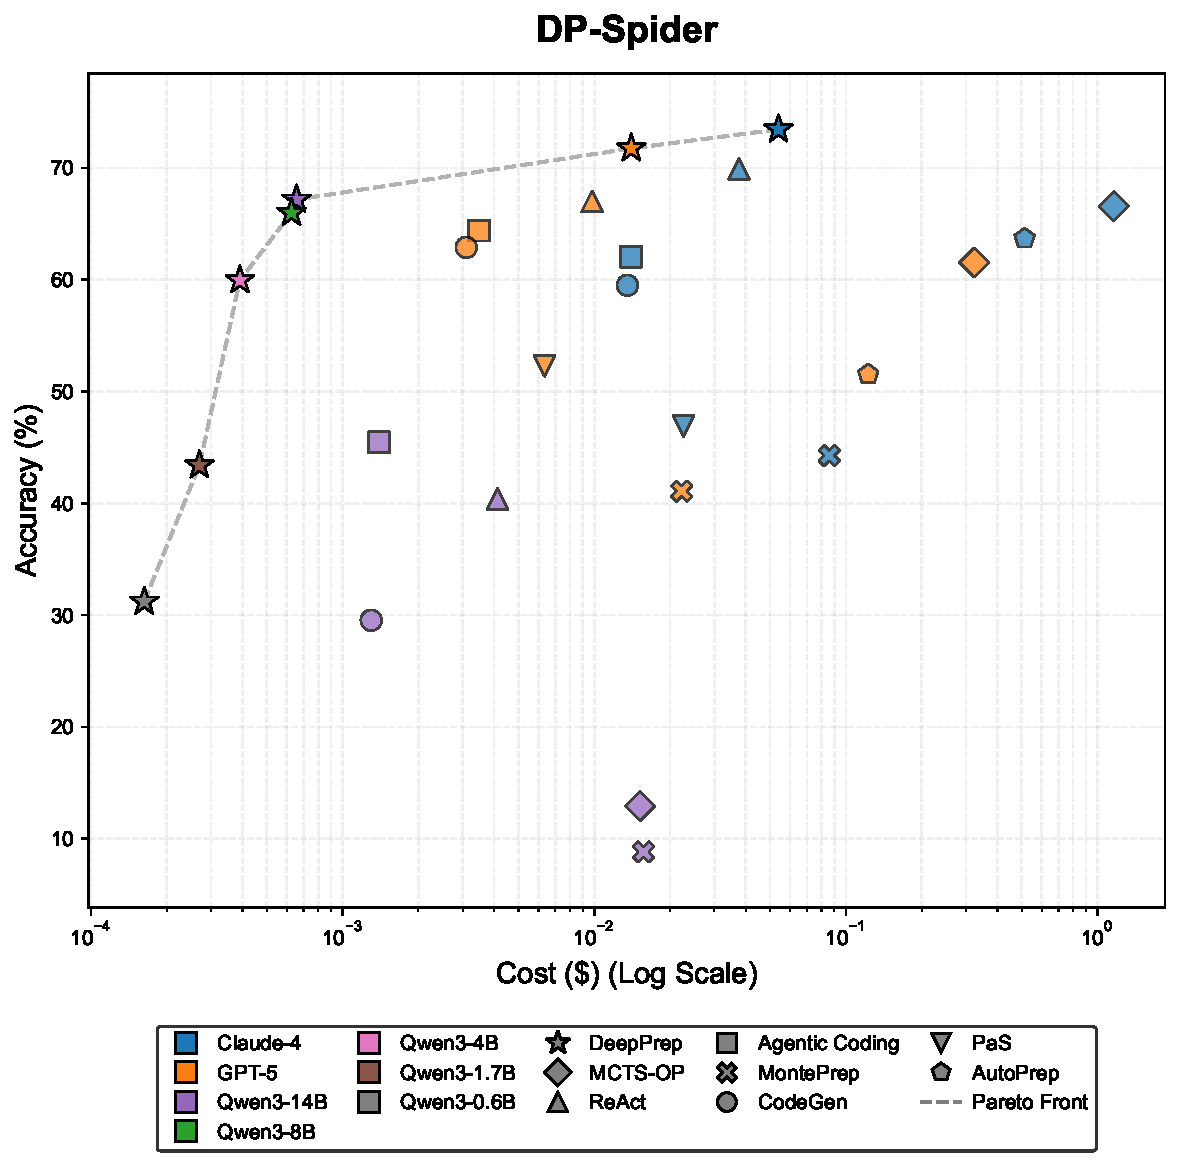
\includegraphics[width=0.99\columnwidth]{plots/plot/pareto_front_spider.pdf}
    \vspace{-1em} 
    \caption{Pareto Front on DP-Spider.}
    \label{fig:pareto_front_spider}
    % \vspace{-1em}
\end{figure}
% \begin{figure}[t]
    \centering
    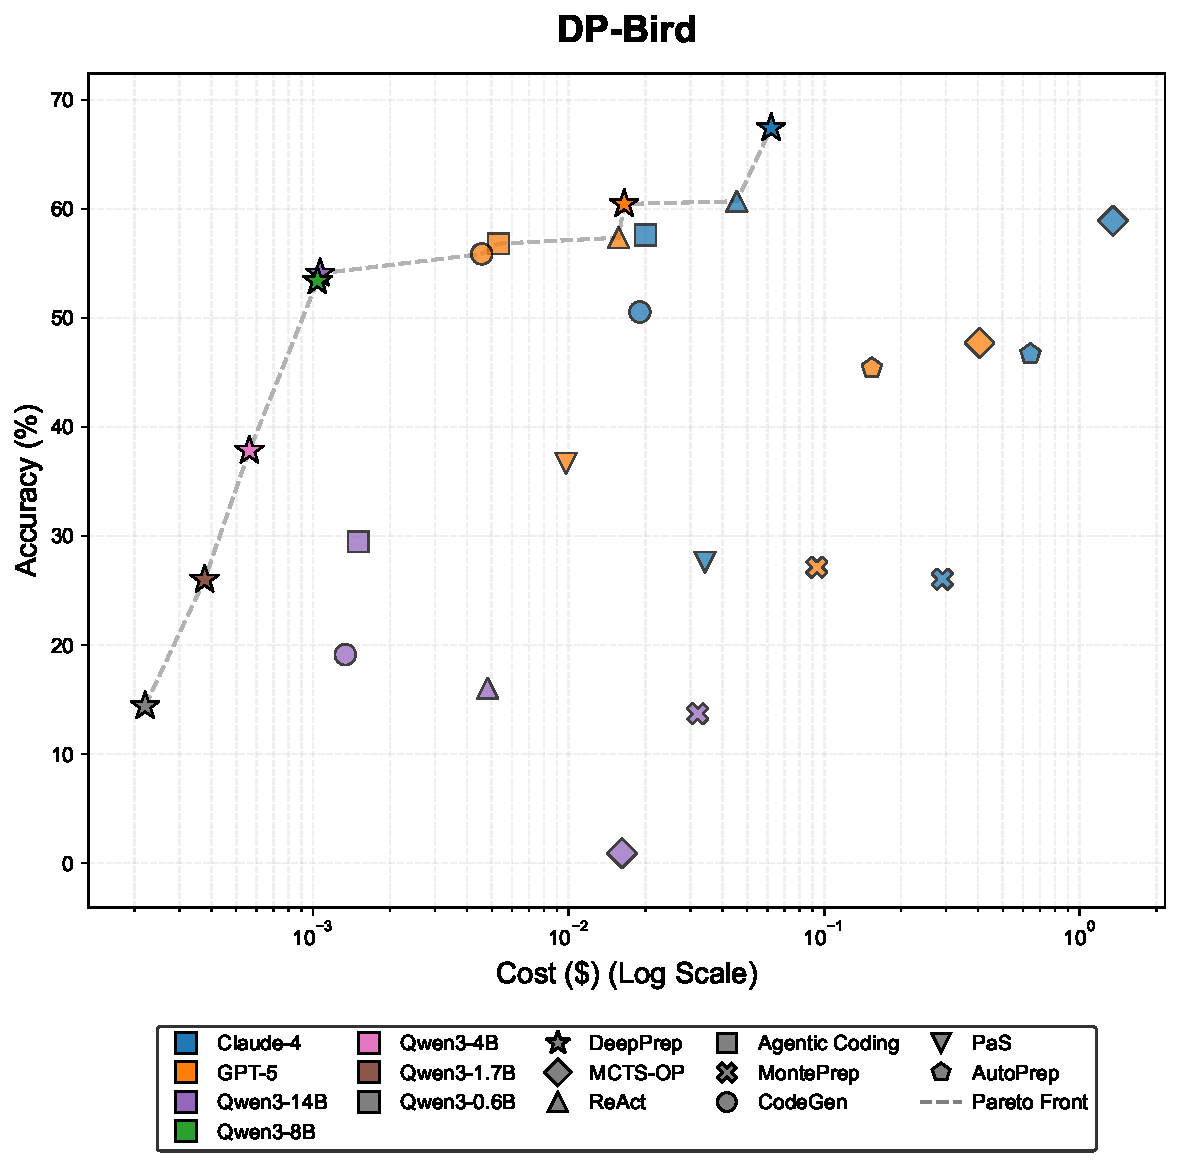
\includegraphics[width=0.99\columnwidth]{plots/plot/pareto_front_bird.pdf}
    \vspace{-1em} 
    \caption{Pareto Front on DP-Bird.}
    \label{fig:pareto_front_bird}
    % \vspace{-1em}
\end{figure}
% \begin{figure}[t]
    \centering
    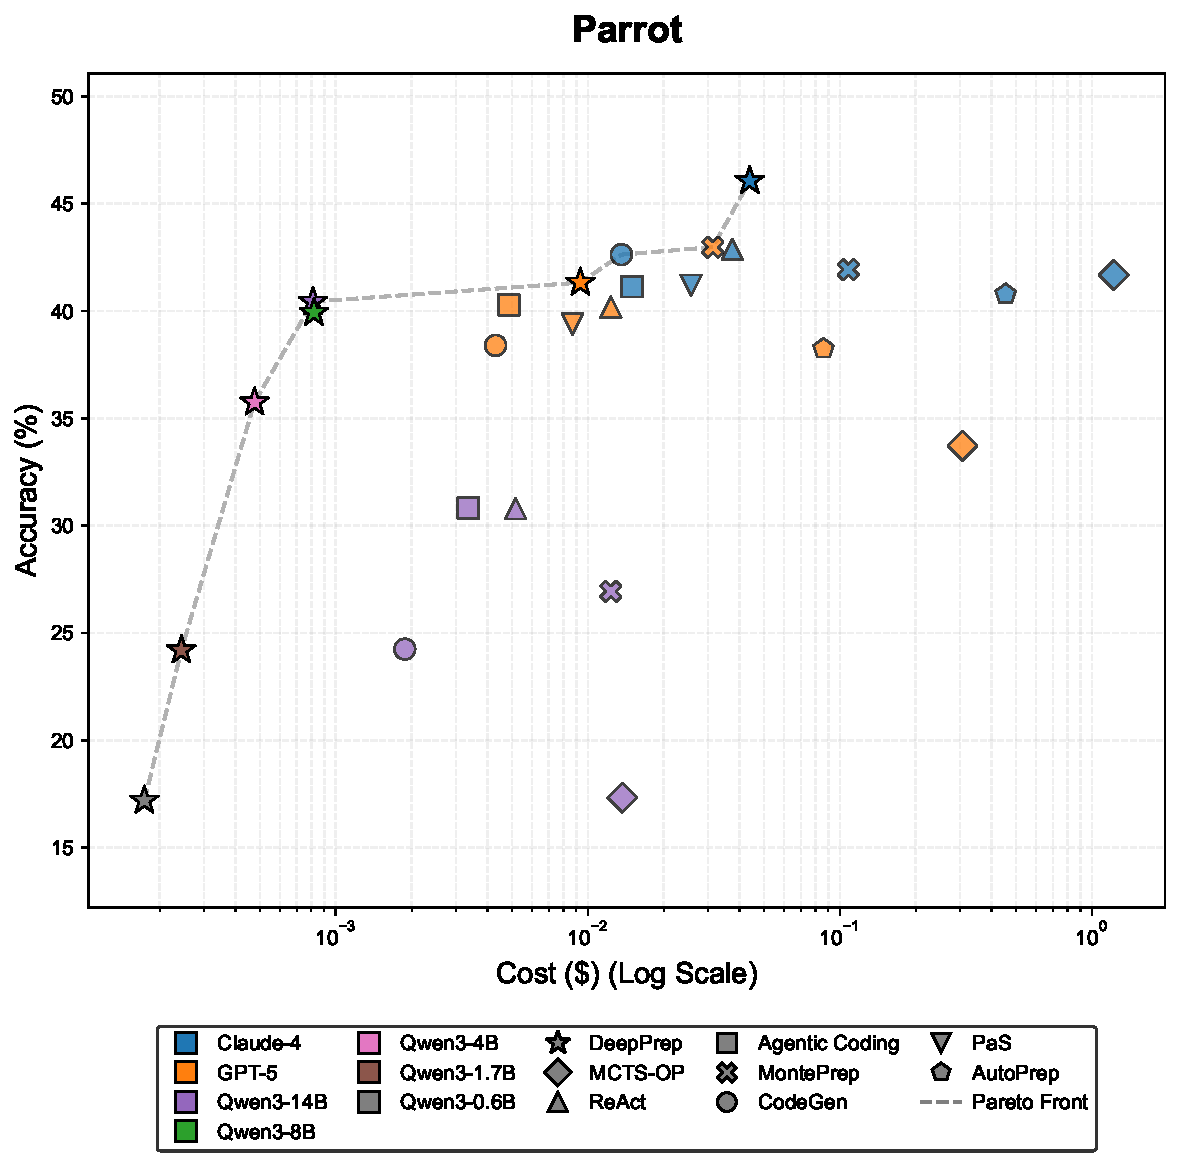
\includegraphics[width=0.99\columnwidth]{plots/plot/pareto_front_parrot.pdf}
    \vspace{-1em} 
    \caption{Pareto Front on Parrot.}
    \label{fig:pareto_front_parrot}
    % \vspace{-1em}
\end{figure}
%!TEX root = ../../main.tex
\begin{figure*}[t]
    \centering 
    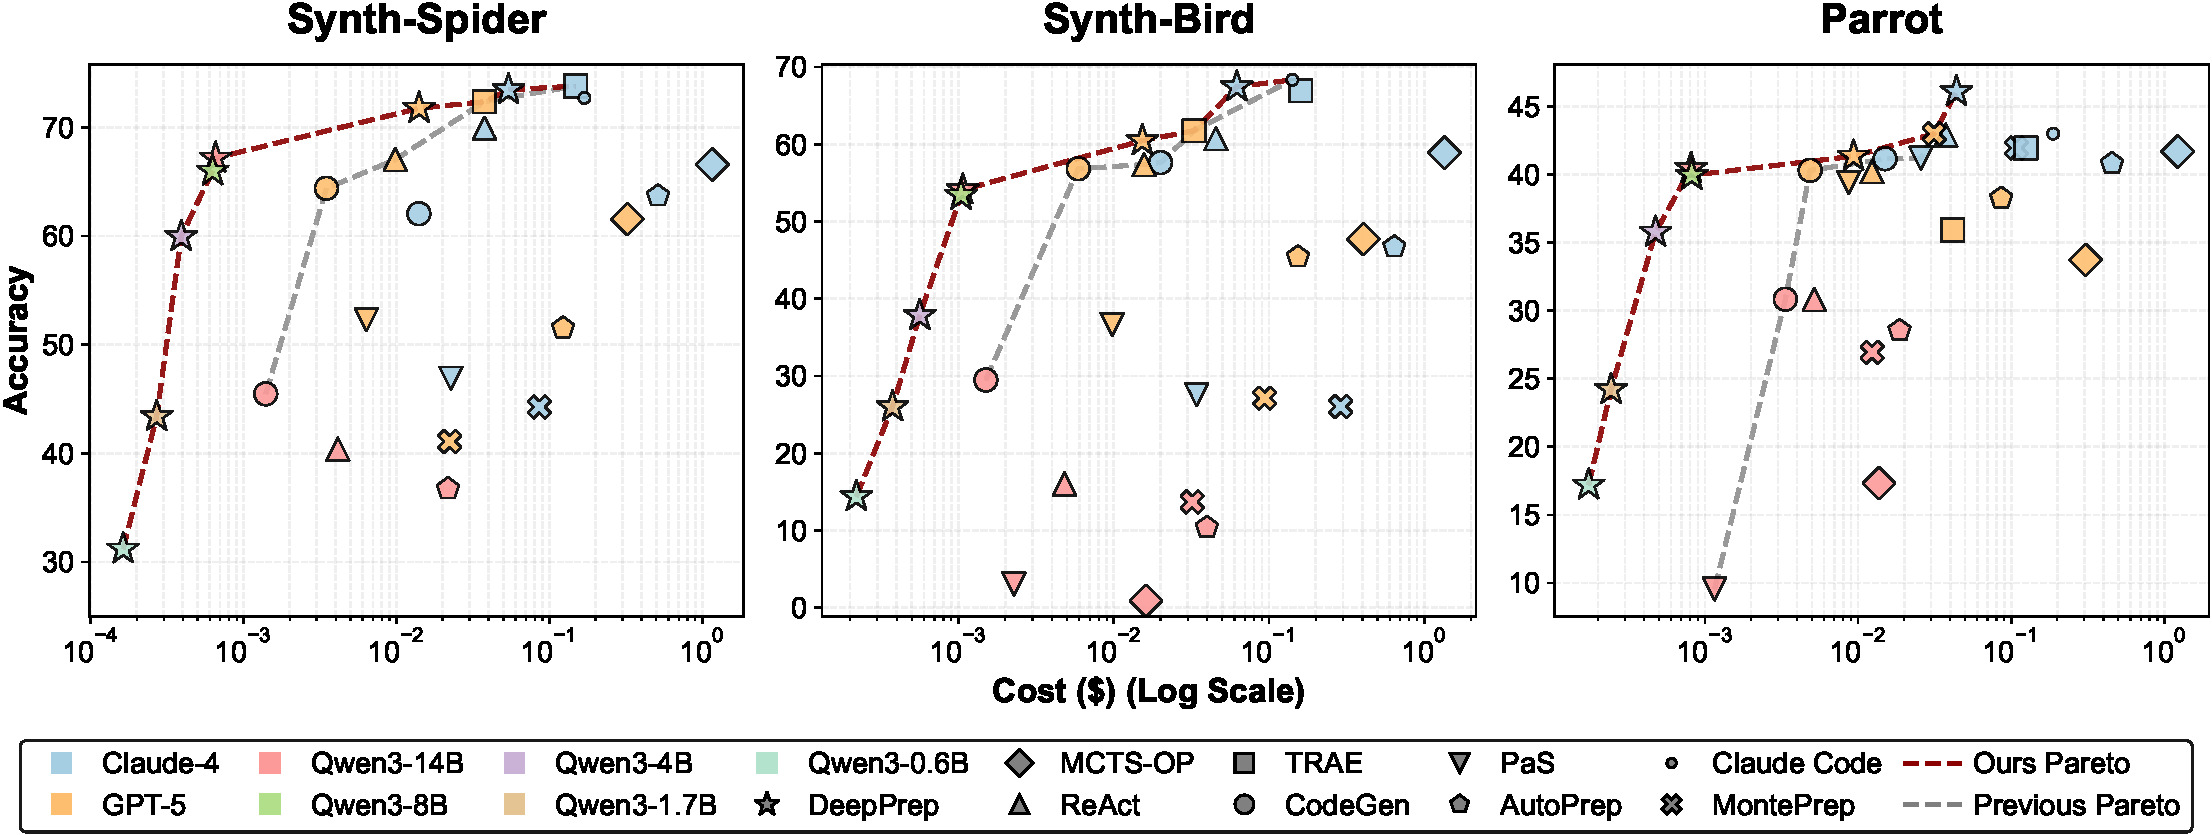
\includegraphics[width=0.7\textwidth]{plots/plot/combined_pareto_front_compare.pdf}
  \vspace{-0.7em}
    \caption{Cost–Accuracy trade-off comparison. Colors represent different LLM backbones, and shapes denote different methods. The red and grey dashed lines indicate the Pareto frontiers of our method and previous baselines, respectively.
    }
    \label{fig:combined_pareto_front_compare}
  \vspace{-1em}
\end{figure*}  



\stitle{Exp-\expnum\label{exp:training_comparison}: Accuracy and Completion Rate Comparison.}
We compare \sys with prompting baselines and training baselines on accuracy and completion rate. 
Results on Qwen3-14B and Qwen3-8B are reported in Table~\ref{tbl:opensource_exp}, as they are strong open-source backbones at two model scales commonly used in code and data tasks. Additional backbone results are presented in later experiments.

\etitle{(1) In-Domain Test.}
\sys achieves the highest accuracy and completion rate across both backbones on the Synth-Spider test set. On Qwen3-14B, it reaches 67.18 accuracy (Table~\ref{subtbl:open_qwen14b}), exceeding the strongest prompting baseline CodeGen by 21.71 points and the strongest training baseline by 5.48 points, with similar gains in completion rate.
% In contrast, the general-purpose data agent DeepAnalyze achieves 35.66 accuracy on the same dataset. 
These gains stem from combining tree-structured exploration with execution-grounded actions, enabling the agent to revise earlier decisions and avoid invalid operator sequences.
% during pipeline construction.

\etitle{(2) Out-of-Domain Test.}
Under the single-source training method, \sys maintains a clear advantage on out-of-domain datasets. On Synth-Bird, \sys (Qwen3-14B) achieves 54.09 accuracy compared with 48.01 for IL, and the 8B model achieves 53.39 versus 43.30. On Parrot, we observe a similar ordering among methods. DeepAnalyze shows much lower performance on Synth-Bird (1.74 accuracy), indicating limited robustness when pipeline length and operator dependencies increase. These results align with our training design, where progressive curriculum and hybrid rewards expose the model to multi-step, feedback-driven reasoning trajectories rather than single-pass program generation.

%\noindent
%\textbf{Exp-\expnum\label{exp:training_comparison}: Accuracy and Complete Rate Comparison.}
%We evaluate the effectiveness of our training strategies by comparing \sys with extensive prompting baselines and training baselines. The results on Qwen3-14B and Qwen3-8B are presented in Table~\ref{tbl:opensource_exp}.

%First, \sys establishes new SOTA results. As shown in Table~\ref{subtbl:open_qwen14b}, \sys (Qwen3-14B) achieves an accuracy of \textbf{67.18} on DP-Spider. This significantly outperforms the best prompting baseline CodeGen by a margin of 21.71 and the best training baselines by a margin of 5.48. Similarly, this advantage is consistent on Complete Rate.
%This substantial improvement validates that the integration of online tree-based agentic reasoning with offline progressive agentic training empowers the agent to autonomously rectify intermediate execution errors and robustly converge to the target schema.
%
%Second, \sys exhibits robust generalization capabilities under the \textit{single-source training, multi-target evaluation} setting. On the complex cross-domain dataset DP-Bird, \sys consistently widens the performance gap against SFT on both backbones. Specifically, \sys (Qwen3-14B) achieves 54.09 accuracy, outperforming SFT (48.01) by a margin of 6.08 points. Similarly, the 8B model achieves 53.39 accuracy, maintaining a strong lead over its SFT baseline (43.30). This indicates that \sys learns the intrinsic reasoning logic of DP rather than merely memorizing schema-specific patterns from the training set. 

%Third, \sys significantly outperforms general-purpose data agents. We observe that DeepAnalyze (Table~\ref{subtbl:open_qwen8b}) struggles in data preparation. While it achieves moderate performance on DP-Spider (35.66), its accuracy collapses to 1.74 on DP-Bird. This highlights the necessity of a dedicated agent for ADP task.
% General agents lack the specialized domain knowledge required to handle multi-hop table transformations. In contrast, \sys leverages high-quality synthesized trajectories to master these domain-specific challenges.

\begin{shaded}
\noindent \textbf{Finding \findingnum: \sys achieves the highest accuracy and completion rate among the compared methods and shows good generalization across datasets.}
\end{shaded}

% \stitle{Finding \findingnum:} \sys achieves the highest accuracy and completion rate among the compared methods and shows good generalization across datasets.

\noindent
\textbf{Exp-\expnum\label{exp:prompting_comparison}: Cost–Accuracy Trade-off Comparison.}
We compare methods under a cost–accuracy trade-off by jointly evaluating accuracy and cost. Figure~\ref{fig:combined_pareto_front_compare} plots prompting baselines and \sys variants across different LLM backbones, and shows two Pareto frontiers: \textit{Previous Pareto}, computed from baselines only, and \textit{Ours Pareto}, computed after adding \sys.

%We further assess \sys's practical utility by jointly considering Exact Matching Accuracy and Inference Cost. Figure~\ref{fig:combined_pareto_front_compare} shows all prompting baselines and \sys variants across different LLM backbones, and overlays two Pareto frontiers: \textit{Previous Pareto}, computed from baselines only, and \textit{Ours Pareto}, computed after adding \sys.

First, \sys lies on or near the Pareto frontier in most settings and extends the frontier across all three datasets. In Figure~\ref{fig:combined_pareto_front_compare}, the \textit{Ours Pareto} curve is shifted toward the upper-left relative to the \textit{Previous Pareto}, meaning that \sys achieves higher accuracy at the same cost, or similar accuracy at lower cost. This appears on Synth-Spider, Synth-Bird, and Parrot, indicating that the cost–accuracy advantage is consistent across datasets and backbones.

Second, \sys reaches accuracy close to strong closed-source baselines at substantially lower cost. On Synth-Spider, \sys (Qwen3-14B) achieves 67.18 accuracy at a very low cost, achieving a comparable accuracy with ReAct on Claude-4 (69.92 accuracy) while reducing cost by about 57$\times$. 
This is attributed to our design that uses structured tree-based reasoning to guide smaller or open models toward valid pipelines with fewer failed executions.

\revise{Third, compared with the agentic coding systems TRAE and Claude Code, \sys achieves comparable accuracy at much lower cost. 
For example, with GPT-5, \sys achieves accuracy comparable to TRAE while reducing cost by 2.7$\times$ on Synth-Spider. This further demonstrates the cost-effectiveness of \sys.}

%Third, \sys remains competitive under more complex scenarios. On Synth-Bird, several search-based baselines show noticeably lower accuracy (\eg MontePrep around 25), whereas \sys continues to appear on the Pareto frontier. A similar trend is observed on Parrot. This suggests that the cost–accuracy behavior of \sys is stable when pipeline length increases.


\begin{shaded}
\noindent \textbf{Finding \findingnum: \sys extends the cost–accuracy Pareto frontier, achieving accuracy close to strong closed-source baselines at substantially lower inference cost.}
\end{shaded}